\documentclass[10pt, t]{beamer}
% \usepackage[UTF8]{ctex}
\usepackage{amsmath}
\usepackage{setspace}
\usepackage{float} 
\usepackage{multido}
\usepackage{multirow}
\usepackage{array}
\usepackage{enumerate}
\usepackage{booktabs}
\usepackage{indentfirst} 
\usepackage[style=mla]{biblatex}
\usepackage{setspace}
\usepackage{subcaption}
\usepackage{hyperref}
\usepackage{textpos}
% \usepackage{fontspec}

% \beamerdefaultoverlayspecification{<+->}
\makeatletter
\let\@@magyar@captionfix\relax
\makeatother

\definecolor{bladerunnerblue}{RGB}{41, 159, 163}
\definecolor{bladerunnerred}{RGB}{194,84,97}
\definecolor{themecolor}{RGB}{25,25,112} 
\definecolor{weak}{RGB}{150,150,150}

\renewcommand{\emph}[1]{{\color{themecolor}\textsl{#1}}}
\newcommand{\alarm}[1]{{\color{bladerunnerred}{#1}}}
\newcommand{\N}{\mathbb{N}}
\newcommand{\R}{\mathbb{R}}
\newcommand{\dom}{\operatorname{dom}}
\newcommand{\myseries}[2]{$#1_1,#1_2,\dots,#1_#2$}
\newcommand{\nullspace}{~\\[15pt]}
\newcommand{\remark}{\textbf{Remark: }}
\newcommand{\question}{\textbf{Question: }}
\newcommand{\scp}[2]{\langle\,#1\,,\,#2\,\rangle} \newcommand{\scpp}{\langle\,\cdot\,,\,\cdot\,\rangle}
\newcommand{\weaken}[1]{{\color{weak}\textit{#1}}}
\newcommand{\underover}[3]{\underset{#2}{\overset{#3}{#1}}}
\renewcommand{\emptyset}{\varnothing}


\usetheme{Madrid}
\setbeamertemplate{navigation symbols}{}

\addtobeamertemplate{frametitle}{}{
\begin{textblock*}{100mm}(0.85\textwidth,-1cm)
\includegraphics[height=1cm]{../../logo.png}
\end{textblock*}}


\usecolortheme[named=themecolor]{structure}

\setbeamertemplate{items}[default]

\hypersetup{
    colorlinks=true,
    linkcolor=themecolor,
    filecolor=themecolor,      
    urlcolor=themecolor,
    citecolor=themecolor,
}

\title{VV186: Honors Mathematics}
\subtitle{Vector Space \& Sequence of Real Functions}
\institute[UM-SJTU JI]{Univerity of Michigan-Shanghai Jiao Tong University Joint Institute}
\author{Xingjian Zhang}

\begin{document}

\begin{frame}
    \titlepage
    \begin{center}
        \includegraphics[height=2cm]{../../logo2.png}
    \end{center}
\end{frame}

\begin{frame}
    \frametitle{Outline}
    \begin{spacing}{1}
        \tableofcontents
    \end{spacing}
\end{frame}

\section{Vector Space}
\subsection{Definition}
\begin{frame}[allowframebreaks]
    \frametitle{Vector Space}
    \begin{figure}[H]
        \centering
        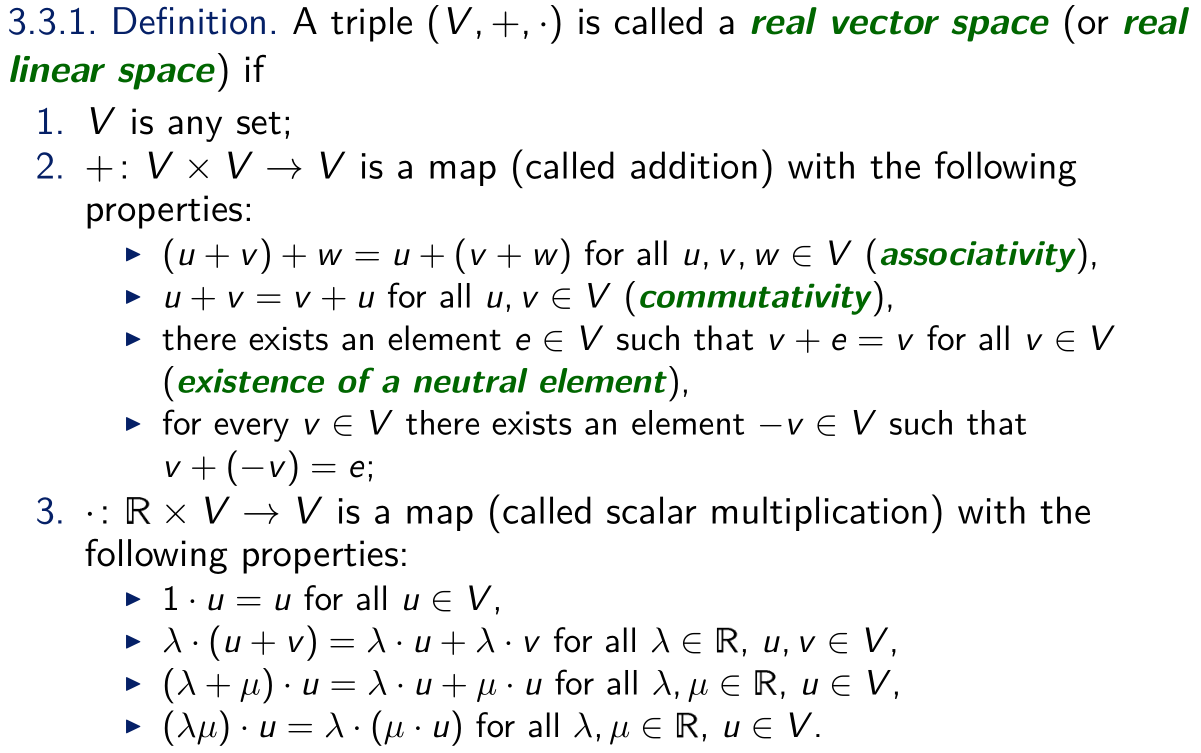
\includegraphics[width=0.9\textwidth]{2020-11-17-19-48-09.png}
    \end{figure}
    \textbf{Remark:}
    \begin{itemize}
        \item 
        Remember all of the 9 properties in the definition.
        \item For both of ``$+$'' and ``$\cdot$'', the \emph{codomain} is $V$. i.e. Both operators should map into original set $V$.
        \item Distinguish clearly a \emph{complex} and a \emph{real} vector space. It is determined by the \emph{domain} of \emph{scalar multiplication}. (Is $\mathbb{C}^n$ a complex or a real vector space?) 
        \item Some common notation:\begin{enumerate}
            \item $\R^n$
            \item $\mathbb{C}^n$
            \item $\mathcal{P}_n$
            \item $C(\Omega , \R)$
            \item $C^k(\Omega , \R)$
            \item $C^\infty(\Omega , \R)$
            \item $\ell^\infty$
            \item $c_0$\footnote[frame]{See Slide p.340 if you forget them.}
        \end{enumerate}
    \end{itemize}
\end{frame}
\subsection{Subspace}
\begin{frame}
    \frametitle{Subspace}

    We defined the \emph{subspace}:
    \begin{figure}[H]
        \centering
        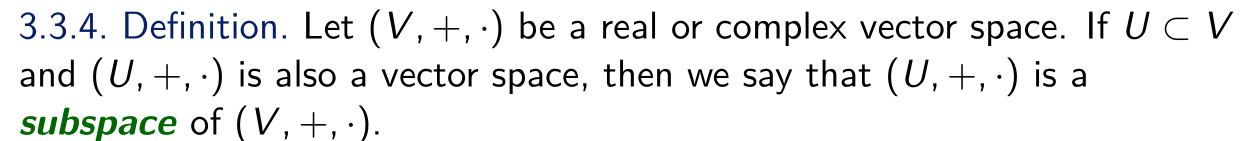
\includegraphics[width=0.9\textwidth]{2020-11-17-20-03-23.png}
    \end{figure}

    We have a simple way to verify a candidate $(U,+,\cdot)$ is indeed a subspace of $(V,+,\cdot)$, given that $(V,+,\cdot)$ is a vector space:
    \begin{figure}[H]
        \centering
        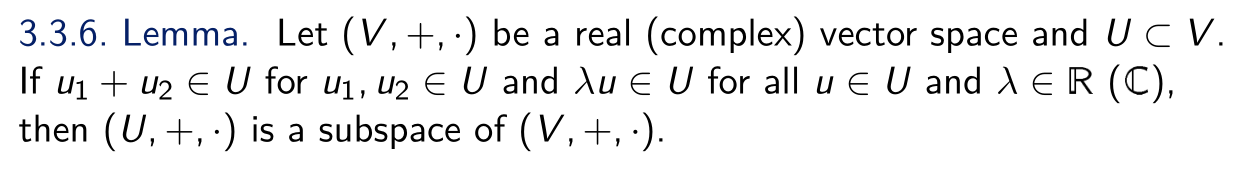
\includegraphics[width=0.9\textwidth]{2020-11-17-20-07-20.png}
    \end{figure}
    True or False? (Give counter-examples or prove.)
    \begin{enumerate}
        \item 
        Given a vector space $V,$ and its two non-empty subspaces $V_{1}, V_{2},$ then $V_{1} \cup V_{2}$ is a subspace of $V$
        \item
        Given a vector space $V,$ and its two subspaces $V_{1}, V_{2},$ then $V_{1} \cap V_{2}$ is a subspace of $V$
    \end{enumerate}
\end{frame}
\subsection{Norm}
\begin{frame}[allowframebreaks]
    \frametitle{Normed Vector Space}

    \emph{Norm} is the ``generalized length function'' in a vector space. We defined it by three properties: 
    \begin{figure}[H]
        \centering
        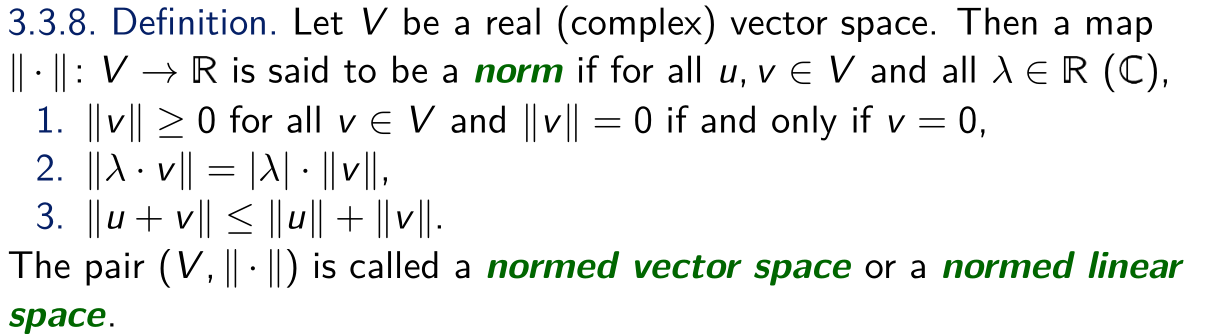
\includegraphics[width=0.9\textwidth]{2020-11-17-20-13-44.png}
    \end{figure}
    \newpage
    \textbf{Remark:}\begin{itemize}
        \item A norm is a (unary) function. So we can naturally investigate into it as considering a function. (e.g. How to prove a norm is continous?)
        \item Any normed vector space can also be considered as a metric space. (How should we define the metric $\rho(x,y)$ according to $\|\cdot\|$?)
        \item Some common notation:\begin{enumerate}
            \item $\|x\|_2$ in $\R^n$ (Euclidean norm)
            \item $\|x\|_p$ in $\R^n$ for $p\in\N^+$
            \item $\|x\|_\infty$ in $\R^n$
            \item $\|(a_n)\|_\infty$ in $\ell^\infty$ or $c_0$
            \item $\|f\|_\infty$ in $C([a,b])$
        \end{enumerate}
    \end{itemize}\nullspace
    True or False? (Give counter-examples or prove.)
    \begin{enumerate}
        \item         Given a vector space $V,$ given two norms $\|\cdot\|_{1}: V \rightarrow \mathbb{R} ;\|\cdot\|_{2}: \mathbb{R} \rightarrow \mathbb{R},$ then the $\|\cdot\|:=\|\cdot\|_{2} \circ\|\cdot\|_{1}$ is a norm of $V$

    \end{enumerate}
\end{frame}

\section{Sequences of Functions}
\subsection{Convergence of Function Sequences}
\begin{frame}
    \frametitle{Pointwise vs. Uniform Convergence}

    \begin{figure}[H]
        \centering
        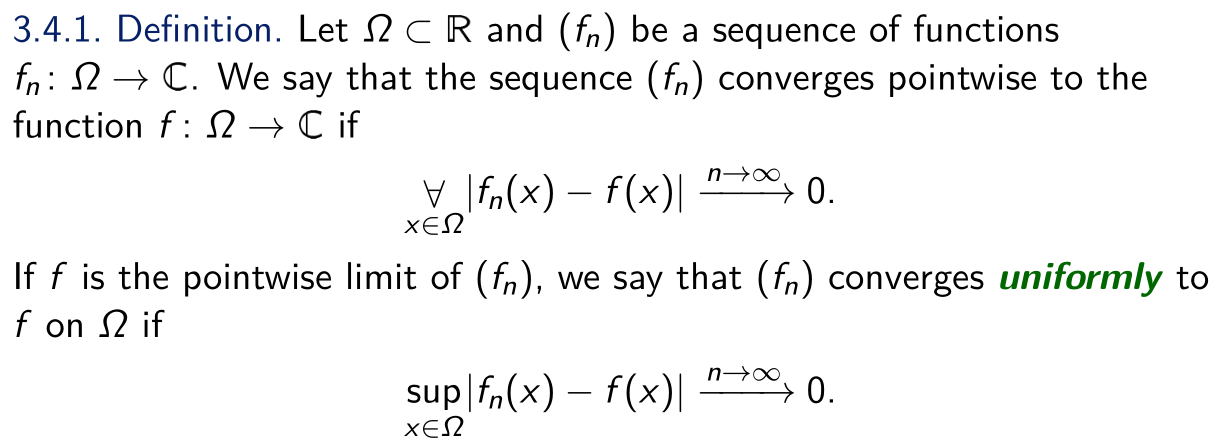
\includegraphics[width=0.9\textwidth]{2020-11-17-20-53-36.png}
    \end{figure}
    \textbf{Remark:}
    \begin{itemize}
        \item What are the differences between them?
        \item What are the relations between them?
        \item Can you come up with some examples to illustrate them?
    \end{itemize}

\end{frame}

\begin{frame}
    \frametitle{How to Calculate}

    Here is a general procedure to find the limit of a function sequence $(f_n)$
    \begin{enumerate}
        \item Fix each $x\in\Omega$, find the pointwise limit of $(f_n)$, denoted by $f$.
        \item Fix each $k\in \N$, find an explicit expression of $\|f_k(x)-f(x)\|$, or an estimate of it.
        \item If 2. $\to 0$ as $k\to \infty$, we have $(f_n)$ converges uniformly to $f$. Otherwise, the convergence is pointwise but not uniform.
    \end{enumerate}
\end{frame}
\subsection{Results}
\begin{frame}
    \frametitle{Results That You Should Know}

    \begin{enumerate}
        \item A uniform convergent sequence of continous functions converges to a continous function.\footnote[frame]{3.4.3. Theorem. Slides p.353}
        \item The metric space $(C([a,b]),\rho)$ is complete, where $\rho(f,g)=\left\|f - g\right\|_\infty$. \footnote[frame]{3.4.4. Theorem. Slides p.355}
    \end{enumerate}
\end{frame}

\begin{frame}[allowframebreaks]
    \frametitle{Sample Solution to Ex.9}

    \begin{figure}[H]
        \centering
        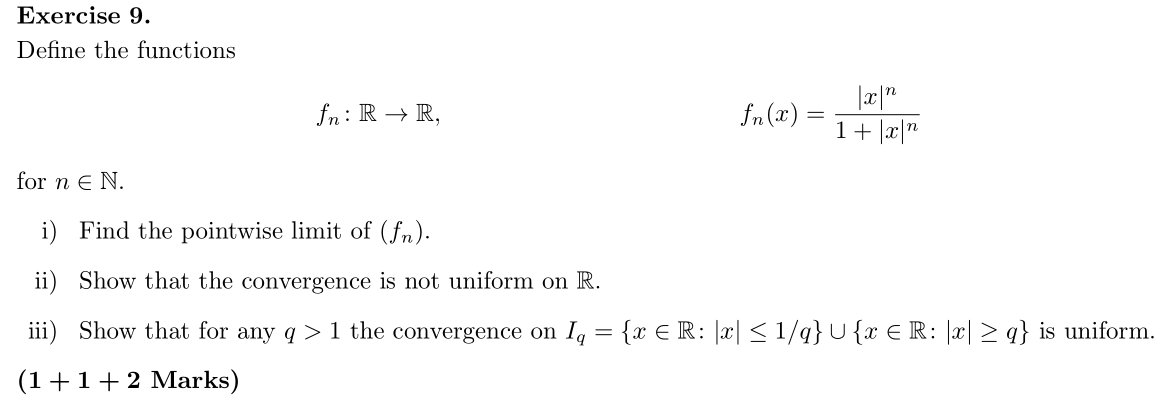
\includegraphics[width=0.9\textwidth]{2020-11-17-21-44-40.png}
    \end{figure}

    \begin{enumerate}[i)]
        \item 
        Fix $x=x_0$,\\
        If $|x_0|<1$, $\underset{n\to\infty}{\lim}|x_0|^n=0$, $\underset{n\to\infty}{\lim}f_n(x_0)=\dfrac{\underset{n\to\infty}{\lim}|x_0|^n}{1+\underset{n\to\infty}{\lim}|x_0|^n}=0$.\\
        If $|x_0|=1$, $\underset{n\to\infty}{\lim}|x_0|^n=1$, $\underset{n\to\infty}{\lim}f_n(x_0)=\dfrac{\underset{n\to\infty}{\lim}|x_0|^n}{1+\underset{n\to\infty}{\lim}|x_0|^n}=1/2$.\\
        If $|x_0|>1$, $\underset{n\to\infty}{\lim}\dfrac{1}{|x_0|^n}=0$, $\underset{n\to\infty}{\lim}f_n(x_0)=\dfrac{1}{1+\underset{n\to\infty}{\lim}\dfrac{1}{|x_0|^n}}=1$.\\[8pt]
        In conclusion, the pointwise limit is $f(x)=\left\{\begin{aligned}
            0 & , & |x|<1 \\
            1/2 & , & |x|=1 \\
            1 & , & |x|>1
            \end{aligned}
            \right.$.
        \item We then show the convergence is not uniform.\\
        \begin{align*}
            \|f-f_n\|_\infty &= \underset{x\in\R}{\sup }|f(x)-f_n(x)|\\
            & \geq |f(3^{-1/n})-f_n(3^{-1/n})|\\
            & = |f_n(3^{-1/n})|\\
            & = 1/4 \nrightarrow 0.
        \end{align*}
        Thus, the convergence is not uniform.
        \item Notice that $f_n(x) = 1-\dfrac{1}{1+|x|^n}$ increases as $|x|$ increases. Similarly, $1-f_n(x) = \dfrac{1}{1+|x|^n}$ decreases as $|x|$ increases. Since 
        \begin{align*}
        \left\|f-f_n\right\|_\infty & = \underset{x\in I_q}{\sup}|f(x)-f_n(x)|\\
        & = \max\left\{\underset{|x|\leq 1/q}{\sup}|f(x)-f_n(x)|,\underset{|x|\geq q}{\sup}|f(x)-f_n(x)|  \right\}\\
        & = \max\left\{\underset{|x|\leq 1/q}{\sup}|f_n(x)|,\underset{|x|\geq q}{\sup}|1-f_n(x)|  \right\}\\
        & = \max\left\{\dfrac{|1/q|^n}{1+|1/q|^n}, \dfrac{1}{1+|q|^n}  \right\}\\
        & = \dfrac{1}{1+|q|^n} \overset{n\to \infty}{\longrightarrow } 0,
        \end{align*}
        the sequence is uniformly convergent on $I_q$.
    \end{enumerate}
\end{frame}

\section{Tips}
\begin{frame}
    \frametitle{Tips}
    Some general tips for the exams:
    \begin{itemize}
        \item Do \textbf{not} stay up too late tonight. You want to have a clear mind at 8 am. tomorrow morning.
        \item The sample exams do not contain exercises regarding vector spaces. However, this does not mean you will not encounter this concept in the exam.
        \item Allocate your time (100mins) wisely in the exam. Finish the easy problems first, focus on tough ones then. The problems are possibly not arranged in the order of difficulty.
    \end{itemize}   
\end{frame}


\begin{frame}
    \frametitle{End}
    \vspace{1.3cm}
    \begin{figure}[H]
        \centering
        
\includegraphics[width=0.8\textwidth]{2020-11-17-22-35-50.png}
    \end{figure}
    
\end{frame}

\end{document}